\documentclass[serif,mathserif,final]{beamer}
\mode<presentation>{\usetheme{Lankton}}


\usepackage[
  orientation=landscape,
  width=40in,height=30in,%size=a0, % paper size
  scale=1.05 % font scale factor
  ]{beamerposter}
 \setbeamertemplate{caption}[numbered] % number figs

% Graphics Path
\usepackage{graphicx}
\graphicspath{{../../figs/}{figs/}}

% OTHER PACKAGE CALLS
\usepackage[utf8]{inputenc}
\usepackage{
  amsmath,amsfonts,amssymb,
  xspace,
  framed,
  siunitx,
  nth,
  physics
}
\sisetup{round-mode = figures, round-precision = 3}
\usepackage{cleveref}

%------ USE BIBLATEX WITH EXTREMELY MINAMALIST STYLE -----
% Use BibLaTeX
\usepackage[
	backend=biber,
	url=false,
	isbn=false,
	doi=false,
	maxnames = 2,
	style=numeric-comp,
	uniquename=false,
	uniquelist=false,
	firstinits=true,
	sorting=none,
	natbib=false,
	isbn=false,
]{biblatex}
\addbibresource{../library.bib}
\renewbibmacro{in:}{}

% One-paragraph bibliography environment
\defbibenvironment{bibliography}
{\list%
  {\printtext[labelnumberwidth]{%
    \printfield{prefixnumber}%
    \printfield{labelnumber}}%
  \ifentrytype{article}{}{}}%
    {\setlength{\leftmargin}{0pt}%
    \setlength{\topsep}{0pt}}%
    \renewcommand*{\makelabel}[1]{##1}}%
  {\endlist}%
{\mkbibitem}

% \mkbibitem just prints item label and non-breakable space
\makeatletter
\newcommand{\mkbibitem}{\@itemlabel\addnbspace}
\makeatother

% Add breakable space between bibliography items
\renewcommand*{\finentrypunct}{\addperiod\space}

% Set fields to clear
\AtEveryBibitem{%
	\clearfield{month}%
	\clearfield{day}%
  \clearlist {language}%why this has to be clear list.....
  \clearfield{pages}%
	\clearfield{pagetotal}%
	\clearfield{eprinttype}%
	\clearfield{eprint}%
	\clearfield{number}%
	\clearfield{volume}%
	\clearfield{issue}%
	\clearfield{name:given}
	\clearfield{name:first}
	\ifentrytype{article}{%
		\clearfield{title}%
	}%
}

%------- GLOSSARIES PACKAGE -------
\usepackage[acronym]{glossaries}
\makeglossaries
\newacronym{wt}{WT}{weather type}
\newacronym{sallj}{SALLJ}{South American low-level jet}
\newacronym{enso}{ENSO}{El Ni\~{n}o-Southern Oscillation}
\newacronym{mjo}{MJO}{Madden-Julian Oscillation}
\newacronym{sacz}{SACZ}{South Atlantic Convergence Zone}
\newacronym{iri}{IRI}{International Research Institute for Climate and Society}
\newacronym{ecmwf}{ECMWF}{European Centre for Medium-Range Weather Forecasts}
\newacronym{s2s}{S2S}{sub-seasonal to seasonal}
\newacronym{eof}{EOF}{empirical orthogonal function}
\newacronym{mos}{MOS}{model output statistics}
\newacronym{xlr}{XLR}{homoscedastic extended logistic regression}
\newacronym{hxlr}{HXLR}{heteroscedastic extended logistic regression}
\newacronym{pcr}{PCR}{principal components regression}
\newacronym{cca}{CCA}{canonical correlation analysis}
\newacronym{sst}{SST}{sea-surface temperature}
\newacronym{scad}{SCAD}{South Central Atlantic Dipole}
\newacronym{lprb}{LPRB}{Lower Paraguay River Basin}

%-- Header and footer information ----------------------------------
\newcommand{\footleft}{Doss-Gollin, J., Á. G. Muñoz, S. J. Mason, and M. Pastén (2018), Heavy rainfall in Paraguay during the 2015-2016 austral summer: causes and sub-seasonal-to-seasonal predictive skill, Journal of Climate, doi:\href{dx.doi.org/10.1175/JCLI-D-17-0805.1}{10.1175/JCLI-D-17-0805.1}.}
\newcommand{\footright}{}
\title{Heavy Rainfall in Paraguay During the 2015-2016 Austral Summer: Causes and Sub-Seasonal-to-Seasonal Predictive Skill}
\author{James Doss-Gollin\inst{1} \quad \'{A}ngel G. Mu\~{n}oz\inst{2} \quad Simon J. Mason\inst{2} \quad Max Past\'{e}n\inst{3}}
\institute
{\inst{1} Columbia Water Center, Columbia University \inst{2} International Research Institute for Climate and Society, Columbia University \inst{3} Direcci\'{o}n de Meteorolog\'{i}a e Hidrolog\'{i}a, Paraguay}

%-------------------------------------------------------------------


%-- Main Document --------------------------------------------------
\begin{document}
\begin{frame}{}
  \begin{columns}[t]

    %-- Column 1 ---------------------------------------------------
    \begin{column}{0.22\linewidth}

        \begin{block}{At a Glance}
  Beginning in Nov. 2015, repeated intense rainfall events associated with mesoscale convective activity caused severe flooding along the Paraguay-Paran\'{a} river system (\cref{fig:study-area}, red box), \emph{displacing over 170000 people}.
  We use a weather typing approch within a diagnostic approach to show that:
  \begin{itemize}
    \item Moisture and energy advection via the South American Low-Level Jet \cite{Marengo:2012cm}, particularly during ``No-Chaco'' events \cite{Vera:2006ib} favored mesoscale convective activity
    \item Strong El Ni\~{n}o favored strong SALLJ but MJO and Atlantic dipole pattern contributed to jet exit region (thus No-Chaco SALLJ events)
    \item Raw S2S model forecasts of rainfall had limited skill beyond 10-15 days, but statistical methods -- particularly the PCR and CCA methods that correct both spatial patterns and magnitudes -- substantially improve forecast skill
  \end{itemize}
  \begin{mdframed}
  \begin{figure}
  	\noindent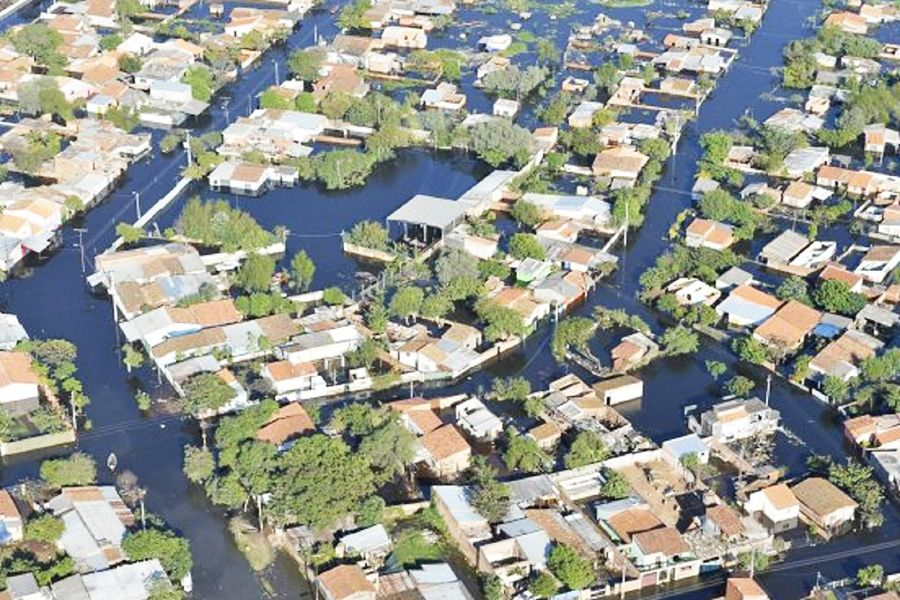
\includegraphics[width=0.45\textwidth]{asuncion-inundaciones.jpg}~
    \noindent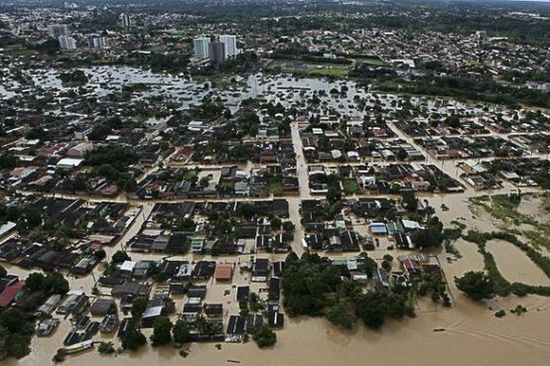
\includegraphics[width=0.45\textwidth]{rio-py-banados.jpg}
  	\caption{
  		Asuncion, Paraguay, 2015-16
  	}
    \label{fig:floods}
  \end{figure}
  \end{mdframed}
\end{block}

        \begin{block}{Observations and Weather Types}
    Observations come from:
    \begin{itemize}
        \item Rainfall:  CPC Global Unified~\cite{Xie:1996ga}
        \item Atmosphere:  NCAR-NCEP Reanalysis II~\cite{Kanamitsu:2002ig}
    \end{itemize}
    We use weather typing~\cite{Munoz:2015dc} to represent daily circulation patterns:
    \begin{enumerate}
        \item Calculate streamfunction $\Psi$ from meridional and zonal wind~\cite{Dawson:2016cu}
        \item Project \SI{850}{\hecto\pascal} streamfunction onto leading 4 EOFs
        \item $K$-means clustering using classifiability index~\cite{Michelangeli:1995es} to generate a single weather type for each day.\\
    \end{enumerate}
    Weather typing simplifies dynamics of daily rainfall but \emph{facilitates analysis of sequences of daily weather patterns}.
    They are associated with patterns that have been well described in the literature; particularly relevant are:
    \begin{enumerate}
        \item \gls{wt}1 represents ``Chaco'' jet event~\cite{Salio:2002ev}
        \item \gls{wt}4 represents ``No-Chaco'' jet events~\cite{Vera:2006ib}
    \end{enumerate}
    \begin{framed}
        \begin{figure}
            \centering
            \noindent\includegraphics[width=\textwidth]{wt_composite.pdf}
            \caption{
                Composite anomalies associated with each weather type.
                Top row (a-f) shows streamfunction anomalies at \SIlist{850}{\hecto\pascal}.
                Strongest 20\% of wind anomaly vectors over the plot area are also shown.
                Bottom row (g-l) shows rainfall anomalies, in units of \si{\milli\meter\per\day}.
                The relative frequency of occurrence of each weather type (in days) is presented on the top of each column.
            }
            \label{fig:weather-type-composite}
        \end{figure}
    \end{framed}
\end{block}


    \end{column}%1

    %-- Column 2 ---------------------------------------------------
    \begin{column}{0.22\linewidth}

      \begin{block}{Observed Circulation Anomalies}
    \begin{framed}
        \begin{figure}
            \centering
            \caption{
                Time series of area-averaged rainfall in the \acrlong{lprb} (\cref{fig:study-area}) for each day of NDJF  2015-16.
                Lines indicate the rainfall value, in units of \si{\milli\meter\per\day}.
                The weather type corresponding to each day is indicated in an adjacent text label.
                Dashed lines blue indicate (from bottom to top) the climatological 50th, \nth{90}, and 99th percentiles of NDJF area-averaged rain over the \acrlong{lprb}.
            }
            \noindent\includegraphics[width=0.9\textwidth]{rain_wt_201516.pdf}
            \label{fig:rain-wtype}
        \end{figure}
    \end{framed}
    During austral summer (NDJF) 2015-16, most heavy rainfall occurred during \glspl{wt} 1 and 4 (\cref{fig:rain-wtype}). 
    Monthly-scale circulation anomalies (\cref{fig:anomaly-ndjf}) show a weak anticyclonic circulation that set up over central Brazil during November 2015 and strengthened into the following month.
    In January 2016 it weakened before returning in February 2016.
    The observed rainfall and circulation anomalies are consistent with the aggregation of the observed weather types shown in \cref{fig:rain-wtype}.
    \begin{framed}
        \begin{figure}
            \centering
            \noindent\includegraphics[width=0.9\textwidth]{anomalies_ndjf1516.pdf}
            \caption{
                Monthly composite anomalies observed during NDJF 2015-16.
                Top row shows streamfunction anomalies at \SI{850}{\hecto\pascal}.
                Bottom row shows rainfall anomalies, in units of \si{\milli\meter\per\day}.
            }
            \label{fig:anomaly-ndjf}
        \end{figure}
    \end{framed}
\end{block}

      \begin{block}{Lower Paraguay River Basin}
  Flat topography limits the river's ability to carry the summer runoff, causing seasonal inundation of the Pantanal and distributing the river discharge in time \cite{Bravo:2011et,Barros:2004bn}.
  During NDJF 2015-16, river stage [height] throughout the Lower Paraguay River Basin reached nearly three times climatological levels (not shown).
  \begin{mdframed}
  \begin{figure}
  	\noindent\includegraphics[width=0.8\textwidth]{study-area.jpg}
  	\caption{
  		Topographical map of the study area.
  	}
    \label{fig:study-area}
  \end{figure}
  \end{mdframed}
\end{block}
  

    \end{column}%2

    %-- Column 3 ---------------------------------------------------
    \begin{column}{0.22\linewidth}

      \begin{block}{S2S Model Forecasts}
    \begin{framed}
        \begin{figure}
            \centering
            \caption{
                Chiclet diagram of ensemble-mean precipitation anomaly forecasts over the \gls{lprb} from ECMWF S2S forecast data, as a function of the forecast target date (horizontal axis) and lead time (vertical axis).
                Time series of daily precipitation over the same area is plotted with $y$-axis inverted.
            }\label{fig:chiclet}
            \noindent\includegraphics[width=\textwidth]{chiclet.pdf}
        \end{figure}
    \end{framed}
    \Cref{fig:chiclet} uses a Chiclet diagram~\cite{Carbin:2016fx} to visualize, as a function of lead time, the time evolution of the uncorrected, ensemble-mean rainfall anomaly forecast, spatially averaged over the \gls{lprb}.
    At lead times greater than about two weeks, the ensemble-mean forecast is slightly wetter than climatology.
    At weather timescales (less than one week), the ensemble-mean successfully predicts the timing and amplitude of the area-averaged rainfall.
    At intermediate timescales, the model successfully forecast the strongest breaks and pauses in the rainfall, such as the heavy rainfall during December 2015 and the dry period during mid-January 2016.
\end{block}

      \begin{block}{Model Output Statistics}
    We explore whether using \gls{mos}~\cite{Glahn:1972iw} can improve the modeled representation of rainfall (\cref{fig:subs-prob-fcst}).
    Specifically, we use: the raw model output (Raw); \gls{xlr}; \gls{hxlr}; \gls{pcr}; and \gls{cca} using 20 years of ECMWF forecasts.
    \Cref{fig:subs-prob-fcst} indicates that better forecasts are obtained when both magnitude and spatial corrections are performed (\gls{pcr} and \gls{cca}).
    The enhanced skill is achieved through the spatial corrections via the EOF-based regressions, which – in contrast with the extended logistic models – use information from multiple grid-boxes,.
    \begin{framed}
        \begin{figure}
            \noindent\includegraphics[width=0.9\textwidth]{mos_forecasts.pdf}
            \caption{
                \Gls{mos}-adjusted S2S model forecasts and skill scores.
                Top row shows the heavy rainfall ($>$\nth{90} percentile exceedance) forecast for 1-7 December 2015 as the odds ratio relative to climatology $\text{odds} = \frac{p}{1-p}\frac{1-p_c}{p_c}$.
                Second row shows the Ignorance score $\text{IGN}=-\log_2 p(Y)$.
                Bottom row shows the 2AFC skill score for each grid cell.
                For all three rows, the grid cells which experienced a \nth{90} percentile exceedance for 1-7 December 2015 are outlined in black.
            }\label{fig:subs-prob-fcst}
        \end{figure}
    \end{framed}
\end{block}


    \end{column}%3


    %-- Column 4 ---------------------------------------------------
    \begin{column}{0.22\linewidth}

      \begin{block}{ENSO, MJO, and Weather Types}
    \begin{framed}
        \begin{figure}
            \centering
            \caption{
                Anomalous probability of occurrence of each weather type concurrent with observance of each MJO and ENSO phase.
                Only values which are significant at $p < 0.10$ are shown.
            }\label{fig:wt-mjo-ensoflooded}
            \includegraphics[width=\textwidth]{wt_mjo_enso.pdf}
        \end{figure}
    \end{framed}
    \gls{wt} 1 occurs more frequently during El Ni\~{n}o years for most \gls{mjo} phases, particularly during phase 2.
    During El Ni\~no years, \gls{wt} 3 - associated with dryness over the \gls{lprb} - occurs less frequently during \gls{mjo} phases 4, 6, and 7, and more often during \gls{mjo} phase 8; this is consistent with the lack of \gls{wt} 3 during December 2015 and the frequent \gls{wt} 3 occurrence in mid-January 2016 (\cref{fig:rain-wtype}).
\end{block}

      \begin{block}{Atlantic-Pacific Interaction and WT4}
    While the occurrence of \gls{wt}1 during NDJF 2015-16 is well explained by ENSO and MJO variability, these features alone do not explain the occurrence of \gls{wt}4, the ``No-Chaco'' jet event.
    Previous studies emphasize the importance of Pacific-Atlantic interaction for forecasting climate effects in this region~\cite{Barreiro:2017ct}.
    A persistent SST dipole in the central southern Atlantic Ocean favors the occurrence of \gls{wt}4 by blocking transient extratropical wave activity coming from the Pacific, facilitating transitions from Chaco jet events (WT 1) to No-Chaco jet events (WT 4) via enhanced low-level wind circulation from southern Brazil towards the Atlantic, and back to north-east Brazil and the Amazon (see \cref{fig:atlantic-pacific}) due to land-sea temperature contrasts.
    Composite analysis (not shown) of months with many \gls{wt}4 occurrences is consistent with the schematic shown here.
    \begin{framed}
        \begin{figure}
            \centering
            \includegraphics[width=\textwidth]{ChacoNoChacojet.pdf}
            \caption{
                Schematics of low-level jet events (red arrows) during austral summer of El Ni\~{n}o years.
            }\label{fig:atlantic-pacific}
        \end{figure}
    \end{framed}
\end{block}


      %-- Block 4-2
      \begin{block}{References}
          \renewcommand*{\bibfont}{\footnotesize}
          \printbibliography[heading=none]
      \end{block}

    \end{column}%1

  \end{columns}
\end{frame}
\end{document}
